\documentclass{book}
\usepackage{graphicx}
\usepackage[english]{babel}
\usepackage{amsthm}
\usepackage{amssymb}
\usepackage{amsfonts}
\usepackage{cancel}
\usepackage{enumerate}
\usepackage[shortlabels]{enumitem}
\usepackage{empheq}
\usepackage{physics}
\usepackage{tikz}
\usepackage[a4paper, margin=1in]{geometry}
\geometry{a4paper, margin=1in}
\usepackage{xcolor}
\usetikzlibrary{arrows.meta}
\usetikzlibrary{angles,quotes}
\graphicspath{ {./images/} }
\usepackage{svg}
\usepackage{subcaption}
\usepackage{bm}
\usepackage{empheq}
\usetikzlibrary{decorations.text}

\usepackage[most]{tcolorbox}
\usepackage{tensor}
%3D
\usepackage{mathtools}
\usepackage{booktabs}
\usepackage{array}
\newcolumntype{C}{>{$}c<{$}}
\usepackage{tikz-3dplot}
\usepackage{appendix}
\usepackage{pgfplots}
\usetikzlibrary{shapes.geometric}
\usetikzlibrary{calc,patterns,angles,quotes}
%Tikz Library
\usetikzlibrary{angles, quotes, intersections}
\usepackage[bb=dsserif]{mathalpha}
\usetikzlibrary{decorations.pathmorphing}

\tikzset{snake it/.style={decorate, decoration=snake}}

\newcommand*\circled[1]{\tikz[baseline=(char.base)]{
		\node[shape=circle,draw,inner sep=2pt] (char) {#1};}}
\newcommand*\widefbox[1]{\fbox{\hspace{2em}#1\hspace{2em}}}

\makeatletter
% the contents of \squarecorner were mostly stolen from pgfmoduleshapes.code.tex
\def\squarecorner#1{
	% Calculate x
	%
	% First, is width < minimum width?
	\pgf@x=\the\wd\pgfnodeparttextbox%
	\pgfmathsetlength\pgf@xc{\pgfkeysvalueof{/pgf/inner xsep}}%
	\advance\pgf@x by 2\pgf@xc%
	\pgfmathsetlength\pgf@xb{\pgfkeysvalueof{/pgf/minimum width}}%
	\ifdim\pgf@x<\pgf@xb%
	% yes, too small. Enlarge...
	\pgf@x=\pgf@xb%
	\fi%
	% Calculate y
	%
	% First, is height+depth < minimum height?
	\pgf@y=\ht\pgfnodeparttextbox%
	\advance\pgf@y by\dp\pgfnodeparttextbox%
	\pgfmathsetlength\pgf@yc{\pgfkeysvalueof{/pgf/inner ysep}}%
	\advance\pgf@y by 2\pgf@yc%
	\pgfmathsetlength\pgf@yb{\pgfkeysvalueof{/pgf/minimum height}}%
	\ifdim\pgf@y<\pgf@yb%
	% yes, too small. Enlarge...
	\pgf@y=\pgf@yb%
	\fi%
	%
	% this \ifdim is the actual part that makes the node dimensions square.
	\ifdim\pgf@x<\pgf@y%
	\pgf@x=\pgf@y%
	\else
	\pgf@y=\pgf@x%
	\fi
	%
	% Now, calculate right border: .5\wd\pgfnodeparttextbox + .5 \pgf@x + #1outer sep
	\pgf@x=#1.5\pgf@x%
	\advance\pgf@x by.5\wd\pgfnodeparttextbox%
	\pgfmathsetlength\pgf@xa{\pgfkeysvalueof{/pgf/outer xsep}}%
	\advance\pgf@x by#1\pgf@xa%
	% Now, calculate upper border: .5\ht-.5\dp + .5 \pgf@y + #1outer sep
	\pgf@y=#1.5\pgf@y%
	\advance\pgf@y by-.5\dp\pgfnodeparttextbox%
	\advance\pgf@y by.5\ht\pgfnodeparttextbox%
	\pgfmathsetlength\pgf@ya{\pgfkeysvalueof{/pgf/outer ysep}}%
	\advance\pgf@y by#1\pgf@ya%
}
\makeatother

\pgfdeclareshape{square}{
	\savedanchor\northeast{\squarecorner{}}
	\savedanchor\southwest{\squarecorner{-}}
	
	\foreach \x in {east,west} \foreach \y in {north,mid,base,south} {
		\inheritanchor[from=rectangle]{\y\space\x}
	}
	\foreach \x in {east,west,north,mid,base,south,center,text} {
		\inheritanchor[from=rectangle]{\x}
	}
	\inheritanchorborder[from=rectangle]
	\inheritbackgroundpath[from=rectangle]
}

\usepackage{etoolbox} % ifthen
\usepackage[outline]{contour} % glow around text
\usetikzlibrary{calc} % for adding up coordinates
\usetikzlibrary{decorations.markings,decorations.pathmorphing}
\usetikzlibrary{angles,quotes} % for pic (angle labels)
\usetikzlibrary{arrows.meta} % for arrow size
\usepackage{xfp} % higher precision (16 digits?)

\renewcommand{\cleardoublepage}{\clearpage}

\title{Introduction to Quantum Mechanics}
\author{Dominik Szablonski}
\newtheorem{law}{Law}
\newtheorem{klaw}{Law}
\newtheorem*{definition}{Definition}
\newtheorem*{theorem}{Theorem}
\newtheorem{postulate}{\textbf{Postulate}}

\pgfplotsset{compat=1.18}
\begin{document}
\maketitle
\tableofcontents
\chapter{Quantum States}
\section{Amplitudes and Interference}
\begin{figure}
	\centering
	\begin{tikzpicture}[scale=0.8]
		\draw (0,5) -- (0,3);
		\draw (0,2) -- (0,1);
		\draw (0,0) -- (0,-2);
		\draw (-4, 1.5) -- (0, 2.5) node[midway, above, sloped] {Path 1};
		\node at (-4, 1.5) {\textbullet};
		\draw (-4, 1.5) -- (0, 0.5) node[midway, below, sloped] {Path 2};
		\draw[->] (0,0.5) -- (3, 1.5);
		\draw[->] (0,2.5) -- (3,1.5);
		\node at (3,1.5) {\textbullet};
		
		\node[below] at (3,1.5) {$x$};
	\end{tikzpicture}
	\caption{An event occurs where a ball can go through one of two paths, each with a different probability $P_1(x)$ and $P_2(x)$ of ending up at position $x$.} \label{fig:ball}
\end{figure}
Quantum mechanics is probabilistic. Let us consider fig. \ref{fig:ball}, where a particle has a probability $P_1(x)$ of travelling through path 1 and ending up at $x$, and a probablility of $P_2(x)$ of travelling through path 2 and ending up at $x$. Classically, the total probablility of the system ending up at $x$ is,
\begin{equation}
	P(x) = P_1(x) + P_2(x),
\end{equation}
however, this is not the case in quantum mechanics. In quantum mechanics, probablities are determined using \textit{amplitudes}, which, unlike probablilities, can be negative and complex. The probablility is then given by,
\begin{equation}
	P(x) = |A(x)|^2 = A^*(x)A(x).
\end{equation}
In order to get the total probablity of event occurring, we must then add the amplitudes together, or rather \textbf{superimpose} them.
\\\\
Let us write the amplitudes for the two paths,
\begin{align}
	A_1(x) & = \sqrt{P_1(x)}e^{i\phi_1} \\
	A_2(x) & = \sqrt{P_2(x)}e^{i\phi_2} \\
	A(x) & = A_1(x) + A_2(x).
\end{align}
The total probability of the particle ending up at $x$ is then,
\begin{equation}
\begin{split}
	P(x) &= |A(x)|^2 = |A_1(x) + A_2(x)|^2\\
	& = |\sqrt{P_1}e^{i\phi_1} + \sqrt{P_2}e^{i\phi_2}|^2 \\
	& = (\sqrt{P_1}e^{i\phi_1} + \sqrt{P_2}e^{i\phi_2})(\sqrt{P_1}e^{-i\phi_1} + \sqrt{P_2}e^{-i\phi_2}) \\
	& = P_1 + P_2 + \sqrt(P_1P_2)\left(e^{i(\phi_1-\phi_2)} + e^{i(\phi_2-\phi_1)}\right) \\
	& = \underbrace{P_1 + P_2}_{\text{Classical Terms}} + \overbrace{2\cos(\theta_1 - \theta_2)\sqrt{P_1P_2}}^{\text{Interference Terms}}. \label{eq:ampadded}
\end{split}
\end{equation}
We see that the approach of adding amplitudes added \textit{interference terms} to the latter half of eq. \eqref{eq:ampadded}. If this term is $+$ive, we get constructive interference, and if it is $-$ive, we get destructive interference.
\section{States of Quantum Systems}
Wavefunctions as we have met previously are only approximation of quantum mechanics. We often talk about \textit{information} in quantum systems, of which there are two types,
\begin{enumerate}
	\item \textbf{What is the system?} This determines the Hamiltonian of the system.
	\item \textbf{What state is the system in?} These are the dynamical properties of the system. These describe the quantum state.
\end{enumerate}
We can denote a configuration of a qunatum system with using \textit{ket} notation, such that,
\begin{equation}
	\ket{\text{configuration}}.
\end{equation}
For a system which can be in more than 1 configuration, its state is in a \textbf{superposition} of all possible configurations. For example, the state of flipping a coin is,
\begin{equation}
	\ket{\psi} = A_H\ket{H} + A_T\ket{T} \label{eq:superpositioncoin}
\end{equation}
where $A_H$ and $A_T$ are the amplitudes corresponding to flipping a heads or a tails.
\\\\
We are able to perform a measurement to find out what state a system is in, and when we do so, we \textbf{collapse the superposition} into the state that we measured. So, lets say we measured a heads - our state would go from that in eq. \eqref{eq:superpositioncoin}, to
\begin{equation}
	\ket{\psi} \to \ket{H}.
\end{equation}
Further, we require the state of the system to be \textbf{normalised}, i.e.,
\begin{equation}
	|A_1|^2 + |A_2|^2 = 1.
\end{equation}
Generally, a quantum state $\ket{\psi}$ can be represented as so,
\begin{align}
	\boxed{\ket{\psi} = \sum_j c_j\ket{j}} \\
	\boxed{\sum_j|c_j|^2 = 1, c_j \in \mathbb{C}}
\end{align}
\subsection{Transforming a quantum state}
Over time a system may evolve, and transform the quantum state. For example, turning the coin over will transform the quantum state of the coin by,
\begin{equation}
	\ket{\Psi} \to A_H\ket{T} + A_T\ket{H}.
\end{equation}
\section{Quantum States as Vectors}
Quantum mechanics is formulated from postulates, such as below,
\begin{postulate}
	The quantum state $\ket{\psi}$ of a system is represented by a normalised vector with complex elements (is a member of a Hilbert space).
\end{postulate}\noindent
We can then simply say that the inner product of a quantum sate vector must equal 1 for it to be normalised. The inner product of a Euclidian space can be defined by the transpose of that vector. I.e, if the vector is $\vb{v}$ with real elements $v_i$,
\begin{equation}
	\vb{v}\cdot\vb{v} = \vb{v}^T\vb{v} = \sum_i v_i^2.
\end{equation}
and its \textit{norm} $|\vb{v}|$ is the square root of this. However, in Hilbert space (complex vector space), the inner product is defined,
\begin{equation}
	\left<\vb{v}, \vb{v}\right> = \sum_i |v_i|^2.
\end{equation}
We must then create a new operation which both takes the transpose of the vector and the conjugate of each element. This is known as the \textbf{Hermitian conjugate}, represented by, $\dag$. It has the followig properties,
\begin{align}
	B^{\dag^{\dag}} & = B\\
	(AB)^{\dag} & = B^{\dag}A^{\dag}.
\end{align}
\subsection{Dual of the quantum state}
We can take the Hermitian conjugate of the quantum state, known as a \textit{dual}. We denote it using a \textit{Bra},
\begin{equation}
	\boxed{\bra{\psi} = \ket{\psi}^{\dag}}.
\end{equation}
From this, we can clearly see that the norm of $\ket{\psi}$ is given by,
\begin{equation}
	|\ket{\psi}| = \sqrt{\vb*{\psi}^{\dag}\vb*{\psi}}
\end{equation}
where $\vb*{\psi}$ is the quantum state vector. It is obvious that the norm may also be written by a combination of the bra and the ket,
\begin{equation}
	\boxed{\braket{\psi}{\psi} =  \vb*{\psi}^{\dag}\vb*{\psi}}. \label{eq:braket}
\end{equation}
If eq. \eqref{eq:braket} does not equal 1, then the state is not normalised. If this is the case, the amplitudes must be scaled by a factor of $$\frac{1}{\sqrt{\braket{\psi}{\psi}}}$$
\subsection{Quantum State Overlaps}
The inner product between two different qunatum states gives their \textbf{overlap}. If we have a state $\ket{\psi} = \sum_i a_i\ket{i}$ and $\ket{\phi} = \sum_j b_j\ket{j}$, their overlap (inner product) is denoted,
\begin{equation}
	\braket{\psi}{\phi} = \sum_i a_i^*b_i \label{eq:define overlap}
\end{equation}
and commutes by,
\begin{equation}
	\braket{\phi}{\psi} = \braket{\psi}{\phi}^*.
\end{equation}
\subsection{Basis States}
Eq. \eqref{eq:define overlap}, carries the implication that, for \textit{configuarations} of a quantum state $\ket{i}$ and $\ket{j}$, the overlap is defined,
\begin{equation}
	\braket{i}{j} = \delta_{ik}
\end{equation}
where Kronecker-Delta ($\delta_{ik}$) is defined,
\begin{equation}
	\delta_{ik} = \begin{cases}
	1 & i = k\\
	0 & i \neq k
	\end{cases}.
\end{equation}
If a set of configuration states are all,
\begin{enumerate}
	\item normalised,
	\item mutually orthogonal,
	\item and span a complete set of mutually exclusive configurations of a quantum state,
\end{enumerate}
they form an \textit{orthonormal basis} for the quantum state of the system.
\subsubsection{Changing of basis}
If a quantum state $\ket{\psi}$ is defined in terms of a set of basis states $\left\{\ket{i}\right\}$, we can redefine the quantum state in terms of a new set basis states $\left\{\ket{j}\right\}$ by,
\begin{equation}
	\ket{\psi} = \sum_j \braket{j}{\psi}\ket{j}.
\end{equation}
\chapter{Measurement}
\begin{postulate}
	When measuring a system in a quantum state $\ket{\psi}$ using a measurement basis that includes a configuration $\ket{\phi}$, the probability amplitude of the measurement outcome of $\ket{\phi}$ is $\braket{\psi}{\phi}$.
\end{postulate}\noindent
When performing measurement, we must first specify the \textit{measurement basis}. Suppose we wish to measure the probablility amplitude of the outcome $\ket{\phi_n}$ of a quantum state $\ket{\psi}$ in the basis $\left\{\phi_i\right\}$. In the case that the quantum state $\ket{\psi}$ is defined in the basis $\left\{\phi_i\right\}$, the measurement of the amplitude is trivial, and we simply read the amplitude off of the quantum state. However, if the quantum state is defined using some other basis $\left\{\Phi_i\right\}$, the probaility amplitude of measuring outcome $\ket{\phi_n}$ in the measurement basis of $\left\{\phi_i\right\}$ is,
\begin{equation}
	A(\text{Outcome} \ket{\phi_n} \text{, in state} \ket{\psi}) = \braket{\phi_n}{\psi}
\end{equation}
as long as each element in the measurement basis $\left\{\phi_i\right\}$ is defined in terms of the basis of the quantum state $\left\{\Phi_i\right\}$.
\section{Stern-Gerlach Experiment}
\begin{figure}
	\centering
	\begin{tikzpicture}
		\node[draw, square] at (0,0) {$\left\{\ket{0}, \ket{1}\right\}$};
		\draw[-Stealth] (-2, 0) -- (-0.8,0) node[above, midway] {$\ket{+}$};
		\draw[-Stealth] (0.8,0) -- (2,-1) node[below, midway, sloped] {$\ket{1}$};
		\draw[-Stealth] (0.8,0) -- (4,0) node[above,midway,sloped] {$\ket{0}$};
		\node[draw, square] at (4.8,0) {$\left\{\ket{0}, \ket{1}\right\}$};
		\draw[-Stealth] (5.6,0) -- (6.8,-1) node[below, midway, sloped] {$\ket{0}$};
		\draw[-Stealth] (5.6,0) -- (6.8,0) node[above,midway,sloped] {$\ket{1}$};
	\end{tikzpicture}
	\caption{A measurement of a particle initially in a $\ket{+}$ state is measured in a $\left\{\ket{0}, \ket{1}\right\}$ basis, and only particles in state $\ket{0}$ can proceed. The particles are measured again in the $\left\{\ket{0}, \ket{1}\right\}$ basis, and only particles in state $\ket{1}$ proceed.} \label{fig:stern gerlach 1}
\end{figure}
\begin{figure}
	\centering
	\begin{tikzpicture}
		\node[draw, square] at (0,0) {$\left\{\ket{0}, \ket{1}\right\}$};
		\draw[-Stealth] (-2, 0) -- (-0.8,0) node[above, midway] {$\ket{+}$};
		\draw[-Stealth] (0.8,0) -- (2,-1) node[below, midway, sloped] {$\ket{1}$};
		\draw[-Stealth] (0.8,0) -- (3.9,0) node[above,midway,sloped] {$\ket{0}$};
		\node[draw, square] at (4.8,0) {$\left\{\ket{-}, \ket{+}\right\}$};
		\draw[-Stealth] (5.7,-0.5) -- (8.8,-0.5) node[above, midway, sloped] {$\ket{-}$};
		\draw[-Stealth] (5.7,0.5) -- (8.8,0.5) node[above,midway,sloped] {$\ket{+}$};
		\node[draw, square] at (9.6,0) {$\left\{\ket{0}, \ket{1}\right\}$};
		\draw[-Stealth] (10.4,0) -- (12.4,-1) node[below, midway, sloped] {$\ket{0}$};
		\draw[-Stealth] (10.4,0) -- (12.4,0) node[above,midway,sloped] {$\ket{1}$};
	\end{tikzpicture}
	\caption{As in fig. \ref{fig:stern gerlach 1}, with an additional intermediary measurement, where the particles in a $\ket{0}$ state are measured in a $\left\{\ket{+}, \ket{-}\right\}$ basis where all particles procede.} \label{fig:stern gerlach 2}
\end{figure}
The Stern-Gerlach experiment essentially confirmed quantum mechanics, and the idea that \textit{measurement affects outcomes of future measurement}. Let us consider a particle which is equally likely to be in one of two states. We can measure these states using one of two basis, $\left\{\ket{0},\ket{1}\right\}$ and $\left\{\ket{+},\ket{-}\right\}$. If the particle's initial state is, 
\begin{equation}
	\ket{\psi} = \ket{+}, \label{eq:init state}
\end{equation}
then we can then make the following measurements,
\begin{enumerate}[start = 1, label={\bfseries Measurement \arabic*:}]
	\item Using the $\left\{\ket{0},\ket{1}\right\}$ basis, only particles in state $\ket{0}$ proceed to the next measurement.
	\item Using Using the $\left\{\ket{+},\ket{-}\right\}$ basis, all particles proceed to the next measurement.
	\item Using the $\left\{\ket{0},\ket{1}\right\}$ basis, only particles in state $\ket{1}$ proceed to the end of the experiment.
\end{enumerate}
We can perform two forms this experiement: one where we omit measurement 2, and one where we perform all 3 measurements, represented by figs. \ref{fig:stern gerlach 1} and \ref{fig:stern gerlach 2} respectively. Let's analyse the results of each variation.
\\
\textbf{Omitting measurement 2}: We begin with all particles in a state as in eq. \eqref{eq:init state}. During measurement 1, the particles have an equal chance to be in state $\ket{0}$ or $\ket{1}$, and since,
\begin{equation}
	|\braket{0}{+}|^2 = \frac{1}{2}
\end{equation}
only half of the particles proceed to measurement 3. All particles are now in state $\ket{0}$, and since,
\begin{equation}
	\braket{0}{1} = 0
\end{equation}
no particles are measured in a $\ket{1}$ state, so no particles make it to the end of the experiment.
\\\\
\textbf{Performing all measurements}: We have the same scenario as in the first experiment. After passing through the measurement 1, only particles in state $\ket{0}$ proceed to measurement 2. When we measure the particles in basis $\left\{\ket{-}, \ket{+}\right\}$, their state will \textit{collapse} to either state. Since $\ket{-}$ and $\ket{+}$ are both equally likely, the wave function of half of the particles will go to,
\begin{equation}
	\ket{\psi} \to \ket{+}
\end{equation}
and the other half,
\begin{equation}
	\ket{\psi} \to \ket{-}.
\end{equation}
At measurement 3, the probability of a particle in a $\ket{-}$ state to collapse to a $\ket{1}$ state is a half, etc. So, only half of the particles which entered the measurement 3 filter proceed to the end of the experiment. And thus, a quarter of the particles which entered the experiment proceed to the end!
\subsection*{Significance of the Stern-Gerlach experiment}
As we have seen, the addition of an intermediate changes the final outcome of an experiment. We have shown that \textit{measurement alone has an observable effect on a quantum system}.
\section{Operators}
A linear operator maps a set of inputs $\mathbb{A}$ to outputs of the same set, i.e.,
\begin{equation}
	\hat{L} \text{ maps } \mathbb{A} \to \mathbb{A}.
\end{equation}
Linear operators are written in terms of the outerproducts of a given orthonormal basis, where the outer product is $\ket{\psi}\bra{\psi}$. To transform an operator to a basis $\left\{j\right\}$, we write,
\begin{equation}
	\hat{L} = \sum_j\sum_{j'}\ket{j}\bra{j}\hat{L}\ket{j'}\bra{j'}.
\end{equation}
The identity operator $\hat{I}$ leaves a state unchanged. The identity operator for a given basis $\left\{j\right\}$ is,
\begin{equation}
	\hat{I} = \sum_J\ket{j}\bra{j}.
\end{equation}
We are able to represent linear operators in a matrix form. This becomes clear when we write,
\begin{equation}
	\hat{L} = \sum_{j,k}c_{jk}\ket{j}\bra{k}
\end{equation}
so that we can write the elements of the matrix form of $\hat{L}$ as,
\begin{equation}
	L_{jk} = c_{jk}.
\end{equation}
\subsection{Functions of linear operators}
We borrow rules from matrices when applying functions to operators, i.e.,
\begin{equation}
	\hat{L}^n = \hat{L}\hat{L}\underbrace{\cdots}_{\substack{n\\\text{ times}}}\hat{L}
\end{equation}
where $\hat{L}$ is applied $n$ times. We can also define more exotic operations such as,
\begin{equation}
	e^{\hat{L}} = \sum_{k=0}^{\infty}\frac{1}{k!}\hat{L}^k
\end{equation}
if a function has a given power series expansion. We note that linear operators are non-commutative,
\begin{equation}
	\hat{A}\hat{B} \neq \hat{B}\hat{A}.
\end{equation}
\subsection{Eigenstates of linear operators}
Every operator has given \textbf{eigenstates} $\ket{v}$ and \textbf{eigenvalues} $\lambda$ which satisfy,
\begin{equation}
	\hat{L}\ket{v} = \lambda \ket{v}
\end{equation}
We can define a hermitian operator $\hat{H}$ which has all the properties of a Hermitian matrix. This operator is diagonal under the basis ascribed by its eigenstates, such that,
\begin{equation}
	\hat{H} = \sum_j \lambda_j\ket{v_j}\bra{v_j}.
\end{equation}
If we have a function $f$ which can be expanded by a power series, then,
\begin{equation}
	f(\hat{H}) = \sum_jf(\lambda_j)\ket{v_j}\bra{v_j}
\end{equation}
\section{Observables and Measurement}
The choice of basis will change which \textbf{observables} we are able to measure. Every observable $\mathcal{A}$ has an associated linear operator $\hat{A}$ which returns its expectation value, such that,
\begin{equation}
	\left<\mathcal{A}\right> = \bra{\psi}\hat{A}\ket{\psi}.
\end{equation}
We define $\hat{A}$,
\begin{equation}
	\hat{A} = \sum_j A_j\ket{a_j}\bra{a_j}
\end{equation}
where $\left\{a_j\right\}$ is a set of configuration states each with a given value $A_j$, which in turn define the observable $\mathcal{A}$. We can write the configuration of the observable more compactly if we treat each term of the operator as its own linear operator. We define a \textbf{projector} to be,
\begin{equation}
	\boxed{\hat{A}_j = \ket{a_j}\bra{a_j}}
\end{equation}
then the operator is,
\begin{equation}
	\boxed{\hat{A} = \sum_j a_j\hat{A}_j}.
\end{equation}
We further require that \textit{linear operators of observables are all Hermitian}.
\\\\
With the above stated, we can now write postulate 2 more formally.
\\
\textbf{Postulate 2.} \textit{A measurement $\mathcal{M}$ of a quantum system is a set of Hermitian linear operators $\left\{\hat{M}_j\right\}$ with non-negative eigenvalues that satisfy,
	\begin{equation}
		\sum_j \hat{M}_j = \hat{I}
	\end{equation}
and the probability of an outcome $j$ when in state $\ket{\psi}$ is,
\begin{equation}
	\boxed{P(\ket{j}) = \braket{\psi_j}{\psi_j}}.
\end{equation}
}
\section{Commutators}
We define the \textit{commutater} of a linear operator as,
\begin{equation}
	\left[\hat{A},\hat{B}\right] = \hat{A}\hat{B} - \hat{B}\hat{A}
\end{equation}
whose output is a linear operator. If this operator is null, i.e., if $\hat{A}\hat{B} = \hat{B}\hat{A}$, we say that the operators $\hat{A}$ and $\hat{B}$ commute.
\begin{theorem}
	If two operators $\hat{A}$ and $\hat{B}$ have a complete set of eigenstates and commute, then there exists a set of simultaneous eigenstates for both operators.
\end{theorem}
\begin{proof}
	Assuming $\hat{A}$ has no degenerate eigenvalues. Let $\ket{v}$ be the eigenstates of $\hat{A}$ and $\lambda$ the eigenvalues. We have,
	\begin{equation}
		\hat{B}\hat{A}\ket{v} = \hat{B}\lambda\ket{v} = \lambda\hat{B}\ket{v}.
	\end{equation}
	Since $\hat{A}$ and $\hat{B}$ commute, we have,
	\begin{equation}
		\hat{B}\hat{A}\ket{v} = \hat{A}\hat{B}\ket{v},
	\end{equation}
	and putting all this together,
	\begin{equation}
		\hat{A}\left(\hat{B}\ket{v}\right) = \lambda(\hat{B}\ket{v}). \label{eq:ajhk}
	\end{equation}
	We have that $\hat{B}\ket{v}$ is an eigenstate of $\hat{A}$ with eigenvalue $\lambda$. Since $\hat{A}$ is not degenerate, then $\hat{B}\ket{v} \propto \ket{v}$, i.e., $\ket{v}$ is an eigenvalue of $\hat{B}$. Thus, if $\hat{A}$ is non-degenerate, then the \textit{eigenstates of $\hat{A}$ are also eigenstaets of $\hat{B}$.}
\end{proof}


\subsection{Compatibility of Measurement}
If an two operators corresponding to two different observables commute, i.e., $\mathcal{A}$ and $\mathcal{B}$ to $\hat{A}$ and $\hat{B}$, then we say that the measurements of those observables are \textit{compatible}, and we can measure them both simulatenously. This is because the operators of the observables correspond to the same eigenbasis.
\\\\
If two operators are non-commutative, then their measurements are \textit{incompatible}. The amount of information we can know about two given incompatible observables is encapsulated by the uncertainty principle. If we define the standard deviation on an observable as,
\begin{equation}
	\begin{split}
	\Delta \mathcal{A} &= \left<\mathcal{A}^2\right> - \left<\mathcal{A}\right>^2 \\
	& = \bra{\psi}\hat{A}^2\ket{\psi} - \left(\bra{\psi}\hat{A}\ket{\psi}\right)
	\end{split}
\end{equation}
then the uncertainty principle states,
\begin{equation}
	\Delta\mathcal{A}\Delta\mathcal{B} \geq \frac{1}{2}\left|\left<\left[\hat{A},\hat{B}\right]\right>\right|
\end{equation}
\chapter{Spin and Real Uses of Quantum Mechanics}
All particles have an intrinsic angular momentum (that differs from orbital angular momentum). Every quantum particle has an associated \textit{spin quantum number} which can take non-negative, half integer values (i.e., 0, $\frac{1}{2}$, 1, $\frac{3}{2}$, etc.) We divide particles into 2 different classes,
\begin{itemize}
	\item \textbf{Fermions}: Half integer spin values.
	\item \textbf{Bosons}: Integer spin values.
\end{itemize}
The spin of a particle corresponds to an axis. The \textit{spin itself} isn't an observable, but \textit{spin along an axis} is. We can define the spin operator on a given axis for any normalised vector $\vb{n}$ as,
\begin{equation}
	\hat{S}_n = n_x\hat{S}_x + n_y\hat{S}_y + n_z\hat{S}_z
\end{equation}
which we can write in the vector form,
\begin{equation}
	\hat{\vb{S}} = \begin{pmatrix}
		\hat{S}_x \\ \hat{S}_y \\ \hat{S}_z
	\end{pmatrix}
\end{equation}
where 
\begin{equation}
	\hat{S}_{\vb{n}} = \hat{\vb{S}}\cdot\vb{n}.
\end{equation}
The spin quantum number $s$ restricts the value of spin a particle can have along any given axis. The spin $S$ of a particle must satisfy,
\begin{equation}
	S \leq \hbar s.
\end{equation}
Furthermore, a particle has \textit{quantised} spin values spaced by $\hbar$. I.e., a spin-1 particle can have spin values,
\begin{equation}
	S = -\hbar, 0, \hbar
\end{equation} 
while a spin-$\frac{1}{2}$ particle can have spin values,
\begin{equation}
	S = -\frac{1}{2}\hbar, \frac{1}{2}\hbar.
\end{equation}
\section{Spin Operators}
We will state properties of spin operators without proof.
\\\\
\textbf{Spin canonical commutation relations} state that for any principle axis $\{j,k,l\}$, the spin operators satisfy,
\begin{equation}
	\left[\hat{S}_j,\hat{S}_k\right] = i\hbar\epsilon_{ijk}\hat{S}_l
\end{equation}
which implies that spin measurements along different axis are incompatible. 
\subsection{Spin-$\frac{1}{2}$ Particles}
\subsubsection{Pauli Operators}
If we work in a basis $\left\{\ket{\uparrow},\ket{\downarrow}\right\}$ corresponding to spin states $\frac{\hbar}{2}$ and $-\frac{\hbar}{2}$ respectively, and using a cartesian axis, we have,
\begin{equation}
	\hat{\vb{S}} = \frac{\hbar}{2}\begin{pmatrix}
		\ket{\uparrow}\bra{\downarrow} + \ket{\downarrow}\bra{\uparrow} \\
		-i\ket{\uparrow}\bra{\downarrow} + i\ket{\downarrow}\bra{\uparrow} \\
		\ket{\uparrow}\bra{\downarrow} - \ket{\downarrow}\bra{\uparrow}
	\end{pmatrix}. \label{eq:spin operators}
\end{equation}
We often use \textit{Pauli operators} $\{\hat{\sigma}_x, \hat{\sigma}_y, \hat{\sigma}_z\}$ which take the form as in eq. \eqref{eq:spin operators} without the $\frac{\hbar}{2}$ factor,
\begin{align}
	\sigma_x = \begin{pmatrix}
		0 & 1 \\ 1 & 0
	\end{pmatrix} && \sigma_y = \begin{pmatrix}
	0 & -i \\ i & 0
	\end{pmatrix} && \sigma_z = \begin{pmatrix}
	1 & 0 \\ 0 & -1
\end{pmatrix}
\end{align}
\subsubsection{Ladder Operators}
These transform spin states by increasing or decreasing the spin along a given axis by 1 unit. We often specify them for the $z$-axis.
\\\\
Let $\ket{m_s}$ be the eigenstate of $\hat{S}_z$ corresponding to the eigenvalue $\hbar m_s$ such that,
\begin{equation}
	\hat{S}_z \ket{m_s} = \hbar m_s \ket{m_s}.
\end{equation}
Then, the spin ladder operators $\hat{S}_+$ and $\hat{S}_-$ for a spin-$s$ particle are as follows,
\begin{align}
		\hat{S}_+ \ket{m_s} = \hbar\sqrt{s(s+1) - m_s(m_s + 1)}\ket{m_s + 1}, \\
		\hat{S}_- \ket{m_s} = \hbar\sqrt{s(s+1) - m_s(m_s - 1)}\ket{m_s - 1}. \label{eq:293}
\end{align}
\textbf{NOTE:} Ladder operators are not Hermitian $\implies$ do not correspond to observables. However, it can be shown,
\begin{equation}
	\hat{S}_+^{\dag} = \hat{S}_-.
\end{equation}
Furthermore, for any spin-$s$,
\begin{equation}
	\hat{S}_{\pm} = \hat{S}_x \pm i\hat{S}_y. \label{eq:290}
\end{equation}
\subsubsection{Spin Eigenstates}
The magnitude of the spin operator is defined,
\begin{equation}
	|\hat{\vb{S}}|^2 = \hat{S}_x^2 + \hat{S}_y^2 + \hat{S}_z^2. \label{eq:129}
\end{equation}
Given the relation by eq. \eqref{eq:290}, combined with eq. \eqref{eq:293} and eq. \eqref{eq:290}, we can show,
\begin{equation}
	\hat{S}^2 \ket{m} = \hbar^2s(s+1)\ket{m}.
\end{equation}
Since this is true for all eigenstaets of $\hat{S}_z$, \textit{every state} of the system is an eigenstate of $\hat{S}^2$ with eigenvalues $\hbar^2s(s+1)$. Thus,
\begin{equation}
	\hat{S}^2 = \hbar s(s+1)\hat{I}.
\end{equation}

\section{Quantum Hamiltonians}
In quantum mechanics, a system's energy is quantised. If the energy of the system is directly measured, the value we find must be consistent with the set described by the \textit{energy spectrum} of the system. We specify this energy spectrum by the Hamiltonian $\hat{H}$. The energy spectrum $\left\{E_i\right\}$ corresponds to the associated energy eigenstates $\left\{\ket{E_i}\right\}$. The eigenvalue equation for these eigenstates takes the form,
\begin{equation}
	\hat{H}\ket{E_i} = E_i\ket{E_i}
\end{equation}
which is also known as the \textit{Time-Independent Schrodinger Equation}.
\\\\
The smallest energy of a system is known as the \textit{ground state} with a corresponding \textit{ground state energy}. All other energy eigenstates are known as \textit{excited states}.
\subsection{Time evolution of a quantum system}
We can use the Hamiltonian to describe the time evolution of a quantum system. By the \textit{Time Dependent Schrodinger Equation},
\begin{equation}
	\boxed{i\hbar \dv{\ket{\psi}}{t} = \hat{H}\ket{\psi}}. \label{eq:tdse}
\end{equation}
If we have a quantum state $\ket{\psi} = \ket{\psi(t)}$, and given we know an initial state $\ket{\psi(t_0)}$, we can obtain the quantum state at any time $t$ by solving  eq. \eqref{eq:tdse}. The general solution is given by,
\begin{equation}
	\ket{\psi(t)} = \exp\left(-\frac{i\hat{H}(t - t_0)}{\hbar}\right)\ket{\psi(t_0)}.
\end{equation}
The solution for the state is much simpler if we work in the energy eigenbasis. If we work in an energy eigenbasis $\left\{\ket{E_i}\right\}$ in an energy spectrum $\left\{E_i\right\}$, and the initial state is defined,
\begin{equation}
	\ket{\psi(0)} = \sum_i c_i\ket{E_i}
\end{equation}
the general solution for the state at time $t$ is,
\begin{equation}
	\ket{\psi(t)} = \sum_ic_i\exp\left(-\frac{iE_it}{\hbar}\right)\ket{E_i}.
\end{equation}
From this we can write postulate 3,
\begin{postulate}
	The time evolution of a closed quantum state is governed by the time dependent Schrodinger equation.
	\begin{equation}
		i\hbar \dv{\ket{\psi}}{t} = \hat{H}\ket{\psi}
	\end{equation}
	with solution,
	\begin{equation}
		\ket{\psi(t)} - \exp\left(-\frac{i\hat{H}t}{\hbar}\right)\ket{\psi(0)}
	\end{equation}
	where $\hat{H}$ is a hermitian operator known as the Hamiltonain.
\end{postulate}
\subsection{Time evolution of expectation values}
The time evolution of quantum expectation is known as \textit{Ehrenfest's theorem}. We first consider the hermitian conjugate of eq. \eqref{eq:tdse},
\begin{equation}
	-i\hbar \dv{\bra{\psi}}{t} = \bra{\psi}\hat{H}. \label{eq:tdse dual}
\end{equation}
We have that the expectation value of an observable $\mathcal{A}$ is given by,
\begin{equation}
	\left<\mathcal{A}\right> = \bra{\psi}\hat{A}\ket{\psi}.
\end{equation}
Taking the time derivative,
\begin{equation}
	\dv{\left<\mathcal{A}\right>}{t} = \dv{\bra{\psi}}{t}\hat{A}\ket{\psi} + \bra{\psi}\hat{A}\dv{\ket{\psi}}{t} + \underbrace{\bra{\psi}\dv{\hat{A}}{t}\ket{\psi}}_{0 \text{, Operators are static}}. \label{eq:kjhlsgh}
\end{equation}
By using eqs. \eqref{eq:tdse} and \eqref{eq:tdse dual}, we can write eq. \eqref{eq:kjhlsgh} by,
\begin{equation}
	\dv{\left<\mathcal{A}\right>}{t} = \frac{i}{\hbar}\bra{\psi}\left[\hat{H},\hat{A}\right]\ket{\psi}.
\end{equation}
We then have that if $\hat{H}$ and $\hat{A}$ commute, i.e., $\left[\hat{H},\hat{A}\right]$, \textit{the expectation of the observable is static}.
\section{Composite Systems}
We divide a system into component subsystems, and assign each of these their own configuration space. We denote the two states of the subsystems $\ket{\psi}$ and $\ket{\phi}$, then the combined state representing the system, $\ket{\Psi}$, is given by,
\begin{equation}
	\ket{\Psi}=\ket{\psi}\otimes\ket{\phi}
\end{equation}
where $\otimes$ is the \textit{tensor product}. 
\\\\
If $\ket{\psi}$ is in a basis $\left\{\ket{e_i}\right\}$ and $\ket{\phi}$ is in a basis $\left\{\ket{e_j}\right\}$, then the basis of the combined state is $\left\{\ket{e_i\otimes e_j}\right\}$ over all possible configurations of $i$ and $j$. This is easily extended for $n$ subsystems.
\\\\
We can extend the tensor product to operators. If we have two operators $\hat{A}_1$ and $\hat{A}_2$ which act on two different subsystems, we can write the operator acting on the total subsystem,
\begin{equation}
	\hat{A} = \hat{A}_1 \otimes \hat{A}_2.
\end{equation}
If we have an operator acting on only a single subsystem, we can find the total operator by performing the tensor product with the identity operator of the other subsystem,
\begin{equation}
	\hat{A} = \hat{A}_1 \otimes \hat{I}_2.
\end{equation}
This leads to the fourth postulate,
\begin{postulate}
	The state space of a composite physical system is the tensor product $\otimes$ of the component physical systems.
\end{postulate}
\subsection{Tensor product mathematics}
We can more clearly see how to compute tensor products by considering vector and matrix representations. Suppose two vectors,
\begin{align}
	\vb{v} = \begin{pmatrix}
		v_1 \\ \vdots \\ v_n
	\end{pmatrix} && \vb{w} = \begin{pmatrix}
	w_1 & \dots & w_m
	\end{pmatrix}
\end{align}
their tensor product is computed by,
\begin{equation}
	\vb{v}\otimes\vb{w} = \begin{pmatrix}
		v_1 \vb{w} \\ \vdots \\ v_n \vb{w}
	\end{pmatrix} = \begin{pmatrix}
	v_1 w_1 & \dots & v_1 w_m \\
	\vdots & \ddots & \\
	v_nw_1 & & v_nw_m
	\end{pmatrix}.
\end{equation}
Similarly for two matrices, 
\begin{align}
	A = \begin{pmatrix}
		a_{11} & \dots &  a_{1j} \\
		\vdots & \ddots & \\
		a_{i1} & & a_{ij}
	\end{pmatrix} && B = \begin{pmatrix}
		b_{11} & \dots &  a_{1l} \\
		\vdots & \ddots & \\
		b_{kl} & & a_{kl}
	\end{pmatrix}
\end{align}
we have,
\begin{equation}
	A \otimes B = \begin{pmatrix}
		a_{11} B & \dots & a_{1j}B \\
		\vdots & \ddots & \\
		a_{i1} B & & a_{ij} B
	\end{pmatrix} = \begin{pmatrix}
	a_{11}b_{11} & \dots & a_{1j}b_{1l} \\
	\vdots & \ddots & \\
	a_{i1}b_{k1} & & a_{ij}b_{kl}
	\end{pmatrix}.
\end{equation}
\textbf{NOTE:} We do not require our vectors or matrices to be the same size in order to perform the tensor product on them.
\section{Entanglement}
There are composite states in quantum mechanics which cannot be written as a product of states of each individual system, i.e., that can only be written as a superposition of basis states. These states are known as \textit{entangled}, and the converse case is known as \textit{seperable}.
\\\\
We can perform measurements on single systems when in a composite system, however we must update the system afterwards. We do this by using projector of the outcome. Suppose $\ket{\Phi}$, written in a basis $\left\{\ket{e_i}\otimes\ket{e_j}\right\}$ is our composite system. The probability of an outcome $\ket{e_1}$ on state 1, we must find the expectation value of $\ket{e_1}\bra{e_1} \otimes \hat{I}$ where $\hat{I}$ corresponds to the first system. The probability is then,
\begin{equation}
	P(\ket{e_1}) = \bra{\Psi} \ket{e_1}\bra{e_1} \otimes \hat{I}\ket{\Psi}.
\end{equation}
Post-measurement, we use the projector to update the composite state, such that,
\begin{equation}
	\ket{\Psi} \to \ket{e_1}\bra{e_1}\otimes \hat{I}\ket{\Psi}.
\end{equation}
\textbf{NOTE:} The state must be renormalised post-update.
\chapter{Higher Dimensional Systems}
\section{Positions and Wavefunctions}
Let us consider a particle present in a region in the spacial $x$-axis between $-w$ and $w$. Let us consider splitting the $x$-axis between these points evenly into $N$ regions. The width $\Delta x$ of each region is given by,
\begin{equation}
	\Delta x = \frac{2W}{N}.
\end{equation}
Let us denote the basis state corresponding to each region as $\ket{n\Delta x}$, where $-N/2 \leq n \leq N/2 -1$. The state of the particle is given by,
\begin{equation}
	\ket{\psi} = \sum_{n=-N/2}^{N/2-1}a_{n\Delta x}\ket{n\Delta x}. \label{eq:psi}
\end{equation}
We have that, for small $\Delta x$, $a_{n\Delta x} \sim a_{(n+1)\Delta x}$. We then have that the probality of finding a particle in a given region,
\begin{equation}
	P(n\Delta x) = \left|a_{n\Delta x}\right|^2
\end{equation}
scaled with $\Delta x$. We may wish to consider the probaility density, rather than the probaility, to describe our system,
\begin{equation}
	p(n\Delta x) = \frac{\ket{n\Delta x}}{\Delta x}. \label{eq:probdens}
\end{equation}
Let us re-define the un-normalised state,
\begin{equation}
	\ket{x_{n\Delta x}} = \frac{\ket{n\Delta x}}{\sqrt{\Delta x}}.
\end{equation}
We then have,
\begin{equation}
	\begin{split}
		& \braket{n\Delta x}{n'\Delta x} = \delta_{nn'} \\
		\implies & \braket{x_{n\Delta x}}{x_{n'\Delta x}} = \underbrace{\frac{\delta_{nn'}}{\Delta x}}_{\text{Dirac Delta}}.
	\end{split}
\end{equation}
Let us then further define,
\begin{equation}
	\psi_{n\Delta x} = \frac{a_n\Delta x}{\sqrt{\Delta x}}.
\end{equation}
From eq. \eqref{eq:psi},
\begin{equation}
	\braket{x_{n\Delta x}}{\psi} = \frac{\braket{n\Delta x}{\psi}}{\sqrt{\Delta x}} = \frac{a_n\Delta x}{\sqrt{\Delta x}} = \psi_{n\Delta x}.
\end{equation}
From eq. \eqref{eq:probdens}, we have that,
\begin{equation}
	p(n\Delta x) = \left|\psi_{n\Delta x} \right|^2,
\end{equation}
which, in the continuous limit becomes,
\begin{equation}
	\ket{\psi} \approx \int\dd{x}\psi(x)\ket{x}. \label{eq:contlim}
\end{equation}
The overlap of two points on the $x$-axis is given by the dirac-delta function,
\begin{equation}
	\braket{x}{x'} = \delta(x-x').
\end{equation}
Taking the overlap of eq. \eqref{eq:contlim} with $\ket{x}$ yields,

\begin{empheq}[box=\widefbox]{equation}
	\begin{split}
		\braket{x}{\psi} & = \int\dd{x'}\braket{x}{x'}\psi(x') \\ & = \int\dd{x'}\delta(x-x')\psi(x') = \psi(x).
	\end{split}
\end{empheq}
The function $\psi(x)$ is an amplitude density known as the wavefunction. Using it, we are able to obtain the probability of finding the particle between two points,
\begin{equation}
	\boxed{P(x_0 \leq x \leq x_1) = \int_{x_0}^{x_1}\dd{x}|\psi(x)|^2 = \int_{x_0}^{x_1}\dd{x}\left|\braket{x}{\psi}\right|^2.}
\end{equation}
Let us state some properties of the wavefunction,
\begin{enumerate}
	\item We require the wavefunction to be normalised, such that,
	\begin{equation}
		|\braket{x}{\psi}|^2 = 1
	\end{equation}
	or alternatively,
	\begin{equation}
		\int_{-\infty}^{\infty} \psi^*(x)\psi(x)\dd{x} = 1.
	\end{equation}
	\item For a wavefunction to be normalisable, it must satisfy the normalisation condition,
	\begin{equation}
		\lim_{x\to \pm x} \left(\psi(x)\right) = 0
	\end{equation}
	\item If $\psi_1$ and $\psi_2$ are both allowed, normalisable wavefunctions of a system, then,
	\begin{equation}
		\psi_3 = \alpha \psi_1 + \beta \psi_2
	\end{equation}
	is also an allowed, normalisable wavefunction of the system.
\end{enumerate}
\section{Continuous Operators}
Continuous operators are often differential operators. Below are some common continous operators,
\begin{align*}
	\text{1D Position Operator} && \text{3D Position Operator} && \text{1D Momentum Operator} && \text{3D Momentum Operator} \\
	\hat{x} = x && \hat{x} = \vb{x} && \hat{p}_{1D} = -i\hbar \pdv{x} && \hat{p}_{3D} = -i\hbar \grad
\end{align*}
it is opssible to construct other operators from these 4 basic operators, such as the Hamiltonian,
\begin{equation}
	\hat{H} = \frac{\hat{p}^2}{2m} + V(\hat{x}) \label{eq:hamiltonian}
\end{equation}
which we can use to construct the continuous Schrodinger wave equation,
\begin{equation}
	\hat{H} \psi(x) = E\psi(x)
\end{equation}
\subsection{Commutation relations}
The following are the canonical commutation relations,
\begin{align}
	\left[\hat{x},\hat{x}\right] = 0 && \left[\hat{p},\hat{p}\right] = 0 &7 \left[\hat{x},\hat{p}\right] = i\hbar.
\end{align}
\subsection{Hermitian Properties}
Continous operators are also hermitina, i.e., $\hat{A}^{\dag} = \hat{A}$. For a discrete system,
\begin{equation}
	\braket{\psi}{\hat{A}\phi} = \braket{\psi\hat{A}^{\dag}}{\phi} = \braket{\hat{A}\psi}{\phi}
\end{equation}
and similarly for a continuous one,
\begin{equation}
	\int_{-\infty}^{\infty}\psi^*\hat{A}\phi \dd{x} = \int_{-\infty}^{\infty}(\hat{A}^{\dag}\psi)^*\phi \dd{x} = \int_{-\infty}^{\infty}(\hat{A}\psi)^*\phi \dd{x}.
\end{equation}
\section{Equation of a free particle}
If we consider a free particle, i.e., without any potential acting on it, we can write the energy eigen-value equation using the Hamiltonian (eq. \eqref{eq:hamiltonian}),
\begin{equation}
	-\frac{\hbar^2}{2m}\pdv{\psi(x)}{x} = E\psi{x}.
\end{equation}
If we write $E$ as,
\begin{equation}
	E = \frac{k^2 \hbar^2}{2m} = \frac{p^2}{2m}
\end{equation}
where $k$ is the wavenumber of our wavefunction. We then obtain a wavefunction for a free particle by a standard solution to the wave equation,
\begin{equation}
	\psi(x) = e^{ikx} = e^{\frac{ip}{\hbar}x}.
\end{equation}
NOTE: This wavefunction is different as it is not normalisable. however it is still allowed to exist.
\subsection{Scattering of free particles}
\begin{figure}
	\centering
	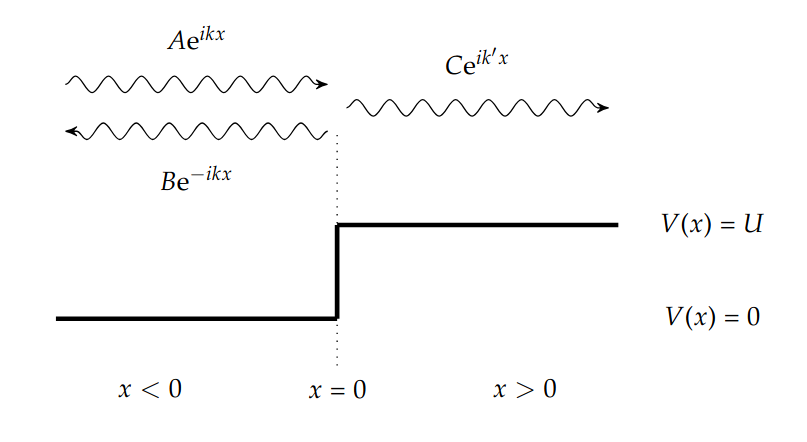
\includegraphics[width=0.75\textwidth]{potential.png}
	\caption{}
	\label{fig:potential barrier}
\end{figure}
Let us now consider a particle beam travelling in space under a potential,
\begin{equation}
	V(x) = \begin{cases}
		0 & x < 0 \\
		U & x \geq 0
	\end{cases}
\end{equation}
with an intial wavefunction,
\begin{equation}
	\psi(x) = Ae^{ikx}
\end{equation}
where it will encounter a potential step at $x = 0$, as in fig \ref{fig:potential barrier} We will have a reflected solution for $x<0$, and a solution where the wave travels past the potential step. We can sum up this wave equation as,
\begin{equation}
	\psi(x) = \begin{cases}
		Ae^{ikx} + Be^{-ikx} & x<0 \\
		Xe^{ik'x} & x \geq 0
	\end{cases}.
\end{equation}
We have a different wavenumber in the region $x \geq 0$ which is related to the potential. We can define this as,
\begin{align}
	E - U = \frac{\hbar^2k'^2}{2m} && \sqrt{k' = \frac{2m(E-U)}{\hbar^2}}.
\end{align}
For conservation of energy, we require boundary conditions which state,
\begin{align}
	\psi(0) \text{ is continuous} \label{eq:conti1} \\
	\eval{\pdv{\psi(x)}{x}}_{0} \text{ is continuous} \label{eq:conti2}.
\end{align}
Applying eq. \eqref{eq:conti1},
\begin{equation}
	A + B = C
\end{equation}
and applying eq. \eqref{eq:conti2},
\begin{equation}
	ik(A - B) = ik'C.
\end{equation}
We then have the relations,
\begin{align}
	B = \frac{k-k'}{k+k'}A && C = \frac{2k}{k+k'}A. \label{eq:relations}
\end{align}
It is tempting to use eq. \eqref{eq:relations} in order to describe the probability of the particle beam becoming reflected off the potential step. However, given that this is a particle beam, we must instead consider the particle flux in order to calculate probabilities. These fluxes are equivalent to the \textit{probability current},
\begin{equation}
	\boxed{j = -\frac{i\hbar}{2m}\left(\psi^*\pdv{\psi}{x} - \psi \pdv{\psi^*}{x}\right)}.
\end{equation}
We can then define the Reflection and Transmission ratios by,
\begin{align}
	\boxed{\mathcal{R} = \frac{j_{\text{ref}}}{j_{\text{inc}}} = \frac{(k-k')^2}{(k+k')^2}} && \boxed{\mathcal{T} = \frac{j_{\text{trans}}}{j_{\text{inc}}} = \frac{4kk'}{(k+k')^2}}
\end{align}
which further satisfy $\mathcal{R} + \mathcal{T} = 1$.
\section{Bound Particles}
\subsection{Infinite Potential Well}
Consider the potential,
\begin{equation}
	V(x) = \begin{cases}
		0 & 0 \leq x \leq L \\
		\infty & \text{Otherwise}
	\end{cases}.
\end{equation}
The Schrodinger equation in this case is identical to that of the free particle,
\begin{equation}
	-\frac{\hbar^2}{2m}\pdv{x}\ket{\psi} = E\ket{\psi}
\end{equation}
but subject to the boundary conditions,
\begin{equation}
	\psi(x) = 0 \text{ for } x \leq 0, x \geq 0.
\end{equation}
Considering the general solution to the wave equation,
\begin{equation}
	\psi(x) = Ae^{ikx} + Be^{-ikx}
\end{equation}
and applying the boundary condition at $x=0$, we find $A = -B$, and,
\begin{equation}
	\psi(x) = A(e^{ikx} - e^{-ikx}) = 2Ai\sin{kx}.
\end{equation}
Applying the boundary condition at $x = L$, we find that the wavenumber is quantised, so that we have integer number of wavelengths,
\begin{equation}
	k = \frac{n\pi}{L} \hspace{1em} n \in \mathbb{Z}^+.
\end{equation}
We are then able to normalise the wavefunction to,
\begin{equation}
	\psi(x) = \sqrt{\frac{2}{L}}\sin(kx).
\end{equation}
We can then find the quantised energy Eigenstates,
\begin{equation}
	E_n = \frac{\hbar^2 n^2 \pi^2}{2mL^2}
\end{equation}
which correspond to the normal modes of the wavefunction.
\subsection{Potential Barriers}
For a potential step, we have that there is a probability that the particle will be found within the potential barrier, such that $\psi(x) \propto e^{-\eta x}$. However, the particle current in the region inside the barrier is 0. 
\subsection{Finite Potential Wells}
For a finite potential well, when the particle is at an energy $0 < E < -U$, we find that the general wavefunction is given by odd and even wavefunctions,
\begin{align}
	\psi(x)_{\text{odd}} = \begin{cases}
		A e^{\eta x} & x < -a\\
		\cos{kx} & |x| < a \\
		Be^{-\eta x} & x > a
	\end{cases}, && \psi(x)_{\text{even}} = \begin{cases}
	A e^{\eta x} & x < -a\\
	\sin{kx} & |x| < a \\
	-Be^{-\eta x} & x > a
	\end{cases}.
\end{align}
we have that,
\begin{align}
	k^2 = \frac{2m(E-U)}{\hbar^2} && \nu^2 = - \frac{2mE}{\hbar^2}.
\end{align}
which we can relate by,
\begin{equation}
	\boxed{k^2 + \eta^2 \frac{2mU}{\hbar^2}}. \label{eq:sol1}
\end{equation}
By considering the continuity boundary conditions, we find that,
\begin{equation}
	\boxed{k\tan{(ka)} = \eta}. \label{eq:sol2}
\end{equation}
We require both eq. \eqref{eq:sol1} and eq. \eqref{eq:sol2} to be solutions. However, no analytical soluton exists. We must then use a graphical solution, as in figure \ref{fig:graph}. The amount of points of interesection represent the number of solutions for the potential well, which indicate the number of eigenstates.
\begin{figure}
	\centering
	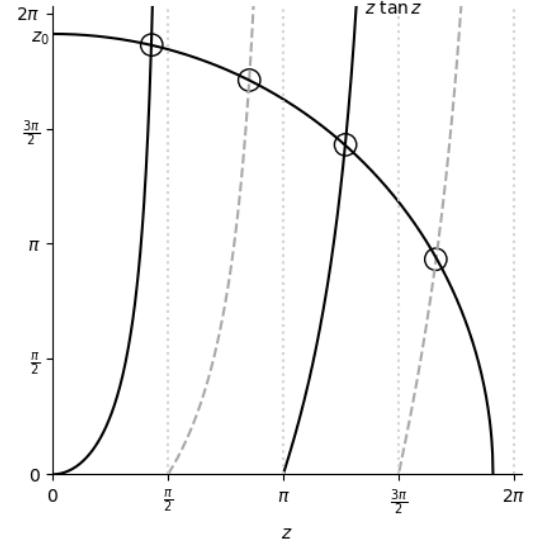
\includegraphics[width=0.4\textwidth]{graph.png}
	\caption{Dashes lines represent odd solutions.}
	\label{fig:graph}
\end{figure}
\section{Expectation Values}
Recall the procedure for findng the expectation value of an observable for a discrete system,
\begin{equation}
	\left<\hat{x}\right> = \bra{\psi}\hat{x}\ket{\psi}.
\end{equation}
We can extend this to a continuous system,
\begin{equation}
	\boxed{\left<\hat{x}\right> = \int_{-\infty} \psi^*\hat{x}\psi \dd{x}}.
\end{equation}
\subsection{Expectation Position of an Infinite Potential Well}
Let us state the position expectation value for position (computation is trivial),
\begin{equation}
	\frac{L}{2} = \left<\hat{x}\right>.
\end{equation}
Let us note that the expectation value is independent of the wavenumber, implying that the expectation value for a particle is the same for all energy states.
\section{Time Evolution}
If we have an intial wavefunction $\psi(x) \equiv \psi(x,t=0)$, with energy eigenfucntions $\left\{\psi_n(x)\right\}$, we can rewrite the time independent wavefunction as a sum of weighted eigenfunctions,
\begin{equation}
	\psi(x) = \sum_n c_n \phi_n(x)
\end{equation}
where the coefficient $c_n$ is determined by,
\begin{equation}
	c_n = \braket{\phi_n}{\psi} = \int_{-\infty}^{\infty} \phi_n^*\psi\dd{x}.
\end{equation}
We can describe the time evolution of the wavefunction by first considering the time evolution of the energy eigenfunctions, which is given trivially by the time-dependent Schoridinger equation, as in the discrete case,
\begin{equation}
	\phi_n(x,t) = \phi_n(x)e^{-\frac{iE_nt}{\hbar}}
\end{equation}
and thus, the time evolution of the wavefunction as a whole is given by,
\begin{equation}
	\psi(x,t) = \sum_n c_n \phi_n(x,0)e^{-\frac{iE_nt}{\hbar}}.
\end{equation}
\subsection{Time evolution of expectation values}
We can simply calculate the time evolved expectation value by considering the inner produce of the time evolved wavefunction,
\begin{equation}
	\left<\hat{x}\right>(t) = \bra{\psi(t)}\hat{x}\ket{\psi(t)}.
\end{equation}
\section{Simple Harmonic Oscillator}
The potentials which we have studied are often not as simple. We often wish to study arbitrary potentials $V(x)$, however the Hamiltonian concerning arbitrary potentials are very difficult to solve. We often employ approximations of continuous potentials, particularly about stationary points $x_0$,
\begin{equation}
	V(x - x_0) = V(x_0) + (x-x_0)\cancelto{0}{\eval{\dv{V}{x}}_{x_0}} + \frac{1}{2}(x-x_0)^2\eval{\dv{V}{x}}_{x_0} + \cdots
\end{equation}
We can neglect the offset of our expansion, which leads to the first term of the expansion to be the quadratic term, which results in the approximation being a \textit{harmonic oscillator}.
\\\\
We can write the hamiltonina of the harmonic oscillator,
\begin{equation}
	\hat{H} = \frac{\hat{p}^2}{2m} + \frac{1}{2}m\omega^2\hat{x}^2.
\end{equation}
This Hamiltonian is very difficult to solve by itself. We can instead reformulate it in terms of the lowering and raising operators, defined by,
\begin{align}
	\hat{a}_+ = \sqrt{\frac{m\omega}{2\hbar}}\left(\hat{x} - i \frac{\hat{p}}{m\omega}\right) && \text{Raising} \\
	\hat{a}_+ = \sqrt{\frac{m\omega}{2\hbar}}\left(\hat{x} + i \frac{\hat{p}}{m\omega}\right) && \text{Lowering}
\end{align}
Let us notice that $\hat{a}_+$ is the Hermitian conjuage of $\hat{a}_-$ and vice versa. Using these definitions, we can rewrite the position and momentum operators,
\begin{align}
	\hat{x} = \sqrt{\frac{\hbar}{2m\omega}\left(\hat{a}_+ + \hat{a}_-\right)} && \hat{p} = \sqrt{\frac{\hbar m\omega}{2}\left(\hat{a}_+ - \hat{a}_-\right)} \label{eq:momentum}
\end{align}
Let us analyse the behaviour of $\hat{a}_+\hat{a}_-$,
\begin{equation}
	\begin{split}
		\hat{a}_+\hat{a}_- & = \frac{m\omega}{2\hbar} \left(\hat{x} - \frac{i\hat{p}}{m\omega}\right)\left(\hat{x} + \frac{i\hat{p}}{m\omega}\right) \\
		& = \frac{m\omega}{2\hbar} \left(\hat{x}^2 + \frac{i}{m\omega}\underbrace{\left[\hat{x}\hat{p} - \hat{p}\hat{x}\right]}_{\left[\hat{x},\hat{p}\right] = i\hbar} +\frac{\hat{p}^2}{m^2 \omega^2}\right).
	\end{split}
\end{equation}
Thus, we can write the Hamiltonian,
\begin{equation}
	\hat{H} = \hbar \omega \left(\hat{a}_+\hat{a}_- + \frac{1}{2}\right).
\end{equation}
Let us now consider the behavour of the lowering and raising operators. We must impose the ladder termination condition on the lowering operator, which states that when acting on a ground state $\ket{0}$,
\begin{equation}
	\boxed{\hat{a}_- \ket{0} = 0}.
\end{equation}
The lowering and raising operators general have a behaviour,
\begin{equation}
	\hat{a}_{\pm}\ket{n} \to \ket{n \pm 1}.
\end{equation}
Let us keep in mind that $\braket{n}{n} = 1$, so we require the lowering and raising operators to preserve normalisation. We then require,
\begin{equation}
	\begin{split}
		\braket{n-1}{n-1} = \bra{n}\hat{a}_+\hat{a}_-\ket{n} & = 1 \\
		\bra{n}n\ket{n} = n\braket{n}{n} = 1
	\end{split}
\end{equation}
thus the normalisation conditions are,
\begin{align}	
	\hat{a}_-\ket{n} = \sqrt{n}\ket{n-1} \\
	\hat{a}_+\ket{n} = \sqrt{n+1}\ket{n+1}.
\end{align}
We can define a Hermitian operator $\hat{N}$,
\begin{equation}
	\hat{a}_+\hat{a}_- =\hat{N}
\end{equation}
which behaves,
\begin{equation}
	\hat{N} \ket{n} = n \ket{n}
\end{equation}
i.e., it tells you the energy level of the observed state.
\subsection{Energy Eigenstates of the Simple Harmonic Oscillator}
Analysing the Hamiltonian more closely, if we attempt to act on an $n$th energy eigenstate,
\begin{equation}
	\begin{split}
	\hat{H} \ket{n} & = \hbar\omega\left(\hat{a}_+\hat{a}_- + \frac{1}{2}\right)\ket{n} \\
	& = \hbar \omega \left(n + \frac{1}{2}\right)\ket{n}
\end{split} 
\end{equation}
therefore, the energy of the $n$th eigenstate is given by,
\begin{equation}
	E_n =  \hbar\omega\left(n + \frac{1}{2}\right) \hspace{1em} n \in \mathbb{Z}^+.
\end{equation}
Let us now analyse the eigenfunctions of the harmonic oscillator. We have that,
\begin{equation}
	\hat{a}_-\phi_0(x) = 0
\end{equation}
where $\phi_0(x)$ indicates the ground state of the energy eigenfunction. We then have,
\begin{equation}
	\begin{split}
	& \pdv{x} \phi_0(x) = -\frac{m\omega}{\hbar}x\phi_0(x) \\
	\implies & \phi_0(x) = Ae^{-\alpha x^2}
\end{split}
\end{equation}
by inspection. By normalising the wavefunction, we find that the ground energy eigenfunction is given by,
\begin{equation}
	\phi_0(x) = \left(\frac{m\omega}{\pi \hbar}\right)^{\frac{1}{4}} e^{-\frac{m\omega x^2}{2\hbar}}.
\end{equation}
Subsequent energy eigenfunctions can be found by using the raising operator.
\subsection{Matrix Treatment of the Simple Harmonic Oscillator}
We can find the matrix form of the raising and lowering operators by considering,
\begin{equation}
	\begin{split}
		\bra{n}\hat{a}_-\ket{m} & = \bra{n}\sqrt{m}\ket{m-1}\\
		& = \sqrt{m} \braket{n}{m-1} \\
		& = \sqrt{m}\delta_{n(m-1)}
	\end{split}
\end{equation}
which we can write in matrix form,
\begin{equation}
	a_- = \begin{pmatrix}
		0 & \sqrt{1} & 0 & 0 & \cdots \\
		0 & 0 & \sqrt{2} & 0 & \cdots \\
		0 & 0 & 0 & \sqrt{3} & \cdots \\
		0 & 0 & 0 & 0 & \cdots \\
		\vdots & \vdots & \vdots & \vdots & \ddots & 
	\end{pmatrix}
\end{equation}
Similarly for the raising operator,
\begin{equation}
	a_+ = \begin{pmatrix}
		0 & 0 & 0 & 0 & \cdots \\
		\sqrt{1} &0&0&0& \cdots \\
		0 & \sqrt{2} & 0&0& \cdots \\
		0 & 0 & \sqrt{3} & 0 & \cdots \\
		0 & 0 & 0 & \ddots &  \\
		\vdots & \vdots & \vdots & & \ddots
		
	\end{pmatrix}
\end{equation}
From this, we can find the matrix form of the momentum operator by eq. \eqref{eq:momentum},
\begin{equation}
	p = \sqrt{\frac{\hbar m \omega}{2}}\begin{pmatrix}
		0 & -i\sqrt{1} & 0 & 0 & \cdots \\
		i\sqrt{1} & 0 & -i\sqrt{2} & 0 & \cdots \\
		0 & i\sqrt{2} & 0& -i\sqrt{3} & \cdots \\
		0 & 0 & i\sqrt{3} & 0 & \cdots\\
		\vdots & \vdots & \vdots & & \ddots & 
	\end{pmatrix}
\end{equation}
\section{First Order Perturbation Theory}
For non-trivial potentials, we can make a first order approximation if the potential can be described as a trivial potential summed with a perturbation. For a potential with energy levels $E_n$ which can be approximated some $0^{\text{th}}$ order potential with energy levels $E^{(0)}_n$ and energy eigenstates $\ket{n^{(0)}}$, plus some perturbation $\hat{H}$, the energy levels of the potential is given by,
\begin{equation}
	E_n = E^{(0)}_n + \bra{n^{(0)}}\hat{H}\ket{n^{(0)}}.
\end{equation}

\appendix
\chapter {Matrix Mathematics}
\section{Eigenvalues and Eigenvectors}
For a matrix $A$, there exists a set of eigenvectors $\left\{\vb{v}_i\right\}$ which are \textit{invariant} under the transformation by the matrix, other than by scaling of the set of eigenvalues $\left\{\lambda_j\right\}$. This can be satisfied by,
\begin{equation}
	A\vb{v} = \lambda \vb{v}.
\end{equation}
If two or more eigenvectors share an eigenvalue they are \textit{degenerate}.
\\\\
Suppose a matrix $A$ with eigenvalue $\left\{\lambda_j\right\}$ and eigenvectors $\left\{\vb{v}_i\right\}$. $\forall$ scalars $a$,
\begin{equation}
	A\vb{v} + aI\vb{v} = \left(\lambda + a\right)\vb{v}.
\end{equation}
We can then calculate eigenvalues by,
\begin{equation}
	\det{A - \lambda I} = 0
\end{equation}
from which the corresponding eigenvectors can be found.
\\\\
If a matrix $A$ and its eigenvalues $\lambda$ is raised to some power $n$, then the eigenvalues of the exponentiated matrix correspond to $\lambda$ raised to the power $n$. Or,
\begin{equation}
	A^n\vb{v} = \lambda^n \vb{v}.
\end{equation}
For a diagonalised matrix, its eigenvalues correspond to the values on the diagonal, and its eigenvectors are the basis vectors of the space.
\section{Hermitian Matrices}
A Hermitian matrix $H$ is one that is invariant under a Hermitian conjugate, i.e.,
\begin{equation}
	H^{\dag} = H.
\end{equation}
Property 1: \textit{The eigenvalues of a Hermitian matrix are real.}
\begin{proof}
	Consider a Hermitian matrix $H$. Take the Hermitian conjugate of its eigenvectors,
	\begin{equation}
		H^{\dag}\vb{v}^{\dag} = \lambda^*\vb{v}^{\dag}.
	\end{equation}
	Since $H$ is hermitian, then,
	\begin{equation}
		\vb{v}^{\dag}H = \lambda^*\vb{v}^{\dag}.
	\end{equation}
	Now consider,
	\begin{equation}
		\vb{v}^{\dag}H\vb{v} = \lambda\vb{v}^{\dag}\vb{v} \label{eq:a1}
	\end{equation}
	and taking the conjugate,
	\begin{equation}
		\vb{v}^{\dag}H\vb{v} = \lambda^*\vb{v}^{\dag}\vb{v}. \label{eq:a2}
	\end{equation}
	We can equate eqs. \eqref{eq:a1} and \eqref{eq:a2},
	\begin{equation}
		\lambda\vb{v}^{\dag}\vb{v} = \lambda^*\vb{v}^{\dag}\vb{v}.
	\end{equation}
	If $\vb{v}$ is non-trivial, $\lambda = \lambda^{*}$ $\therefore \lambda \in \mathbb{R}$.
\end{proof}\noindent
Property 2: \textit{The eigenvectors of a Hermitian matrix corresponding to different eigenvalues are orthogonal.}
\begin{proof}
	Let $\lambda_1$ and $\lambda_2$ be the eigenvalues of a Hermitian matrix $H$, with eigenvectors $\vb{v}_1$ and $\vb{v}_2$ respectively. We have,
	\begin{align}
		\vb{v}_2^{\dag}H\vb{v}_1 &= \lambda_1 \vb{v}_2^{\dag}\vb{v}_1 \label{eq:a3}\\
		\vb{v}_1^{\dag}H\vb{v}_2 &= \lambda_2 \vb{v}_1^{\dag}\vb{v}_2.\label{eq:a4}
	\end{align}
	Taking the Hermitian conjugate of eq. \eqref{eq:a4}, 
	\begin{equation}
		v_2^{\dag}H\vb{v}_1 = \lambda_2\vb{v}_2^{\dag}\vb{v}_1.\label{eq:a5}
	\end{equation}
	Equating eqs. \eqref{eq:a3} and \eqref{eq:a5},
	\begin{equation}
		\lambda_1\vb{v}_2^{\dag}\vb{v}_1 = \lambda_2\vb{v}_2^{\dag}\vb{v}_1.
	\end{equation}
	Given $\lambda_1 \neq \lambda_2$, we require $\vb{v}_2^{\dag}\vb{v}_1 = 0$ $\therefore$ $\vb{v}_1$ and $\vb{v}_2$ are orthogonal.
\end{proof} \noindent
A consequence of of property 2 is that a Hermitian matrix can always be diagonalised under a basis transformation.
\chapter{Postulates of Quantum Mechanics}
Below are all the postulates of quantum mechanics, stated in full.
\begin{enumerate}
	\item The quantum state $\ket{\psi}$ of a system is represented by a normalised vector witih complex elements.
	\item A measurement $\mathcal{M}$ of a quantum system is a set of Hermitian linear operators $\left\{\hat{M}_i\right\}$ with non-negative eigenvalues taht satisfy
	\begin{equation}
		\sum_i \hat{M}_i = \hat{I}.
	\end{equation}
	The born rule states that the probability of obtaining an outcome $i$ when in state $\psi$ is,
	\begin{equation}
		P(i) = \bra{\psi}\hat{M}_i\ket{\psi}.
	\end{equation}
	\item The time evolution of a closed quantum system is governed by the Schroedinger equation,
	\begin{equation}
		i\hbar \dv{\ket{\psi}}{t} = \hat{H}\ket{\psi}
	\end{equation}
	where $\hat{H}$ is a Hermitian operator known as the Hamiltonian. The Schroedinger equation has solution,
	\begin{equation}
		\ket{\psi(t)} = \exp\left(-i\frac{\hat{H}(t-t_0)}{\hbar}\right)\ket{\psi(t_0)}.
	\end{equation}
	\item The state space of a composite physical system is the tensor product $\otimes$ of the component physical systems.
\end{enumerate}
\end{document}
